\section{The Large Hadron Collider}
\label{sec:lhc}
(describe the accelerator complex, proton bunches, c.m. energy, all experiments, run periods, inst. and integrated lumi, Run 3 and HL-LHC plans) \\

\onehalfspacing CERN accelerator complex is a progression of machines namely Linac 2, Proton Synchrotron Booster (PSB), Proton Synchrotron (PS), Super Proton Synchrotron (SPS) and Large Hadron Collider (LHC) as shown in Fig. 1 that accelerate particles mainly protons to increasingly higher energies of 50 MeV, 1.4 GeV, 25 GeV, 450 GeV and 14 TeV respectively. Each machine is used to increase the energy of particle before the beam is injected into to the next machine. Linear accelerator (Linac2) is the starting point for protons used in various experiments at CERN. After proton energy reaches 50 MeV, protons enter PSB which further increases its energy before they are injected into PS which takes up its energy to 25 GeV. After reaching 25 GeV, protons enter SPS which further increases its energy to 450 GeV. The protons are finally transferred to two beam pipes of LHC kept at very high vacuum.  \\ 

The Large Hadron Collider (LHC) is the most powerful particle accelerator in the world primarily build to collide protons and heavy ions at 7, 8, 13 and 14 TeV during different LHC run period. The LHC consists of a 27 kilometre ring of superconducting magnets producing strong magnetic field which is used to guide particle beams along the LHC ring. Proton beam made up of bunches travelling in opposite directions kept in two ultrahigh vacuum tubes are accelerated close to the speed of light using time dependent electric field produced by radiofrequency cavities before they collide at four interaction points along the LHC ring where ATLAS, ALICE, CMS and LHCb detectors are placed. \\

The first proton beam was successfully maneuvered around the LHC ring in September 2008 that marked the beginning of Run 1 with proton beams colliding at 7-8 TeV center-of-mass energy and this run period ended in 2013. Run 2 started in 2015 with protons colliding at 13 TeV center-of-mass energy and continued till October 2018. Run 3 is expected to begin at the start of March 2022 and High Luminosity (HL)-LHC phase is expected to begin in mid-2027. Proton Synchroton (PS) is responsible for providing proton bunches spaced 7 metres (25 ns) apart with each bunch containing more than 100 billion protons. The maximum number of bunches reached with the beam preparation method used during Run 2 is 2556. The number of protons in the colliding bunches, time of separation between the bunches and effective area of the bunch which depend on the rms transverse bunch size along horizontal and vertical directions is one of the ways to calculate instantaneous luminosity (L_{inst}). \\

Luminosity is a key performance parameter of an accelerator as it is a measure of number of collisions. Luminosity can be categorized into two types: instantaneous and integrated luminosity. Instantaneous luminosity is defined as the number of collisions occuring per second in per centimeter square area while integrated luminosity is obtained by integrating instantaneous luminosity over a time interval. Both are very important variables as they are used to obtain the number of collision events. During Run 1, peak value of LHC instantaneous luminosity was $0.77 \times 10^{34} \: cm^{-2} s^{-1} $ with $30 \: fb^{-1}$ integrated luminosity. During Run 2, LHC instantaneous luminosity reached a peak value of $1.58 \times 10^{34}  \: cm^{-2} s^{-1}$ with $150 \: fb^{-1}$ integrated luminosity as shown in Fig. 2. At the end of Run 3, we expect to achieve an integrated luminosity  of $300 \:fb^{-1}$ while Phase 2 HL-LHC is expected to collect $3000 \:fb^{-1}$ of data as shown in Fig. 3 thereby increasing luminosity by a factor of 10 beyond the LHC's design value. \\


\begin{figure}[H]
  \centering
  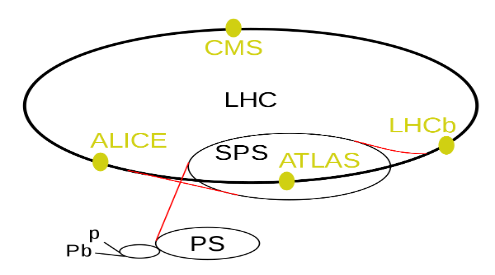
\includegraphics[width=0.8\columnwidth]{./LHCcomplex.png}
  \caption{\onehalfspacing Diagram of the LHC accelerator complex located in Geneva, Switzerland. Four interaction points are shown for the ALICE, ATLAS, LHCb and CMS experiments.}
  \label{fig:LHC}
\end{figure}


\begin{figure}[H]
  \centering
  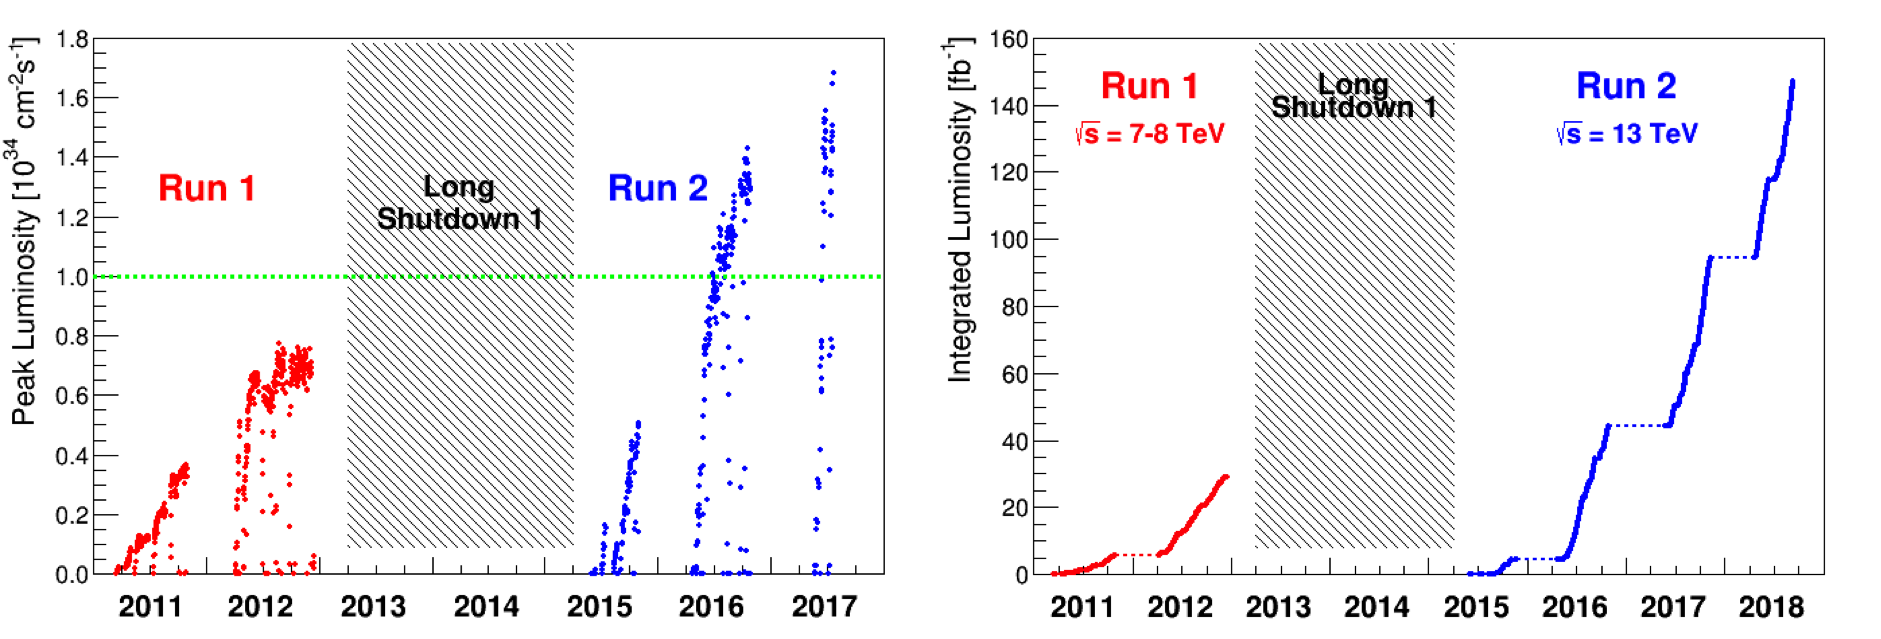
\includegraphics[width=1 \columnwidth]{./run1-2_lumi.png}
  \caption{\onehalfspacing Left: Instantaneous luminosities for Run 1 and Run 2 period. Right: Integrated luminosities for Run 1 and Run 2 period.}
  \label{fig:LHClumi}
\end{figure}


\begin{figure}[H]
  \centering
  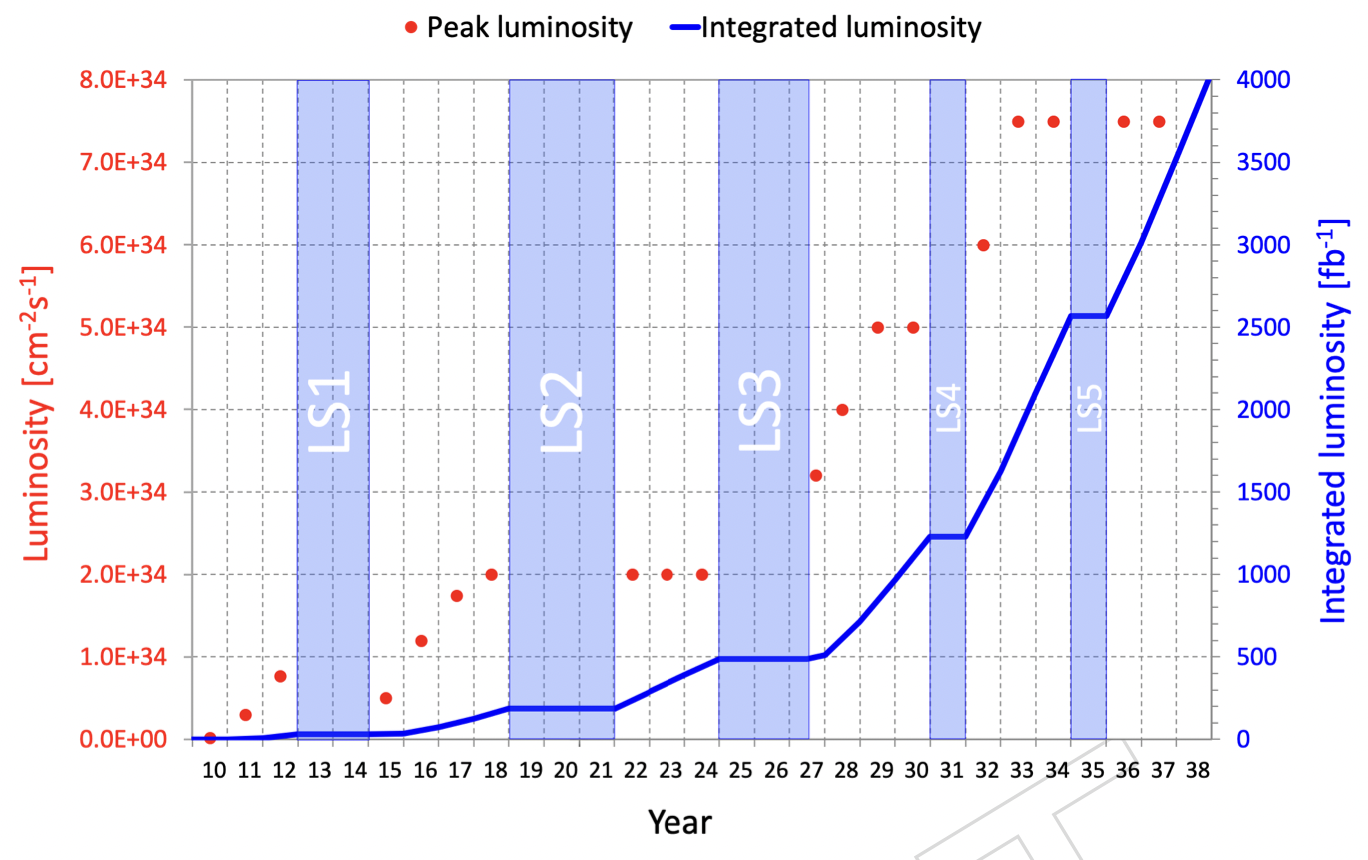
\includegraphics[width=0.7 \columnwidth]{./HLLHCLumi.png}
  \caption{ \onehalfspacing Projected performance of the LHC until 2038, which shows the preliminary dates for prolonged stops (LS1, LS2, LS3, LS4, LS5) of the LHC and luminosities. Red points show instantaneous luminosity $(L_{inst})$ while the blue line shows integrated luminosity. \cite{collaborations2019report}.}
  \label{fig:LHCPlans}
\end{figure}
